\documentclass[border=2pt,tikz]{standalone}



\usetikzlibrary{decorations.pathmorphing}
\begin{document}
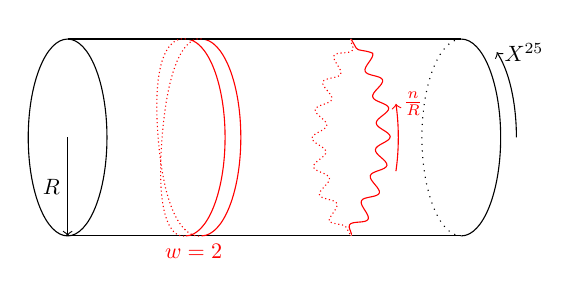
\begin{tikzpicture}[remember picture]
\draw (0,0) ellipse (0.5 and 1.25);
\draw (0,-1.25) -- (5,-1.25);
\draw (5,-1.25) arc (-90:90:0.5 and 1.25);
\draw[red] (1.5,-1.25) arc (-90:90:0.5 and 1.25);
\draw[red] (1.7,-1.25) arc (-90:90:0.5 and 1.25);
\draw [dotted] (5,1.25) arc (90:-90:-0.5 and 1.25);
\draw (0,1.25) -- (5,1.25);
\draw[->] (0,0)  to  node [left,scale=0.8] {$R$}  (0,-1.25);



\draw [->, domain =0:60] plot ({.5* cos (\x )+5.2} , {1.25* sin (\x )}) node [right,scale=0.8] {$X^{25}$} ;


\draw [red,densely dotted] plot [smooth, tension=2] coordinates {(1.5,1.25) (1.15,0) (1.7,-1.25)};
\draw [red,densely dotted] plot [smooth, tension=2] coordinates {(1.7,1.25) (1.2,0) (1.5,-1.25)};

\node [red,scale=0.8] at (1.6,-1.45) {$w=2$};
\draw [->, domain =-20:20,red] plot ({.5* cos (\x )+3.7} , {1.25* sin (\x )}) node [right,scale=0.8] {$\frac nR$} ;

\tikzset{
    demo decoration/.style={
        white,
        postaction={draw=red,decorate,decoration=#1}
    }
}
   
    \draw[demo decoration=snake](3.6,-1.25)to[bend right](3.6,1.25);
    \draw[demo decoration=snake,densely dotted](3.6,1.25)to[bend right](3.6,-1.25);
    
    
    
\end{tikzpicture}
\end{document}